\section{Results}
\label{sec:results}

\subsection{Earlier baselines establish the context}
Table~\ref{tab:baselines} reports selected within-cohort contrasts from the earlier information study and baseline extension. Time weighting improves a frequency baseline, and temporal features retain value conditional on other model features. Clustering and association rules show no stable overall benefit beyond the full model. An early local rule signal does not clearly replicate in the later cohort. A quota-constrained reranker selects weight zero on validation, leaving the base ranking unchanged; its equal confirmation score is a structural identity, not evidence that the proposed change succeeded.

\begin{table}[tbp]
  \centering
  \caption{Earlier within-cohort evidence. Differences are in percentage points of Recall@10. The first two rows use the information cohort; the last two use the separate baseline-extension cohort.}
  \label{tab:baselines}
  \small
  \begin{tabularx}{\linewidth}{@{}XrX@{}}
    \toprule
    Comparison & Difference & Interpretation \\
    \midrule
    Time decay minus frequency & $+3.73$ & Time information helps \\
    Full minus no temporal features & $+3.89$ & Conditional temporal value \\
    TIFU minus same-time personal vector & $+0.61$ & Small neighbor contribution \\
    Full minus adapted TIFU & $+1.96$ & Strong learned baseline \\
    \bottomrule
  \end{tabularx}
\end{table}

The independent TIFU-KNN adaptation follows documented author-code time weighting and restricts recommendations to historical candidates. It is not a reproduction of the paper's full-basket benchmark~\citep{hu2020}. Its neighbor contrast uses the same selected personal time vector. Because the rule and neighbor experiments begin from different personal baselines, their differences cannot be attributed solely to information representation.

\subsection{History-group composition changes the comparison}
In the memory study, users with 3--5 historical orders have mean Recall@10 of 67.97\%, compared with 50.11\% for users with at least 16 orders. Across all users in those groups, mean historical candidate counts are 27.66 and 111.48, respectively. The raw long-minus-short recall gap is therefore $-17.86\pp$, but the two groups differ substantially in the size of the recommendation task.

We restrict comparisons to common historical-covariate cells and apply identical pooled cell weights to each history group. Strata use either candidate count alone or candidate count together with historical mean basket size. Figure~\ref{fig:history} separates the change in population from the subsequent reweighting. Count-only strata retain 5,970 of 7,472 eligible users (79.90\%); count-plus-basket-size strata retain 3,424 (45.82\%). Same-support raw gaps remain negative at $-5.68$ and $-8.06\pp$, whereas standardized gaps are $+13.15$ and $+4.21\pp$. Their conditional marginal 95\% intervals are $[+11.10,+15.13]$ and $[+0.90,+7.15]\pp$.

\begin{figure}[tbp]
  \centering
  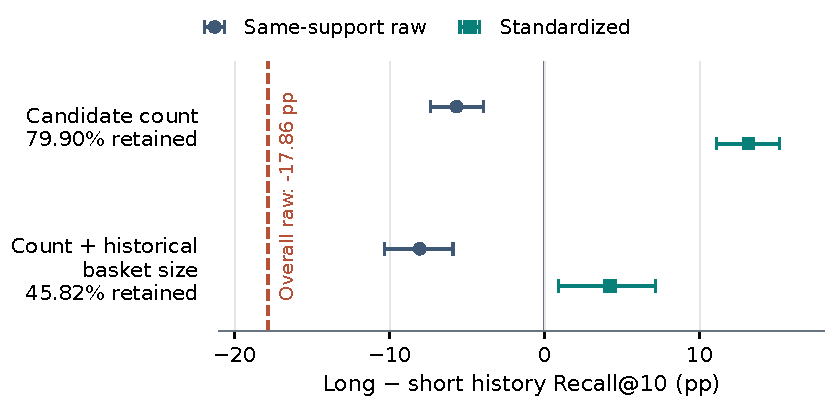
\includegraphics[width=0.95\linewidth]{history_composition.pdf}
  \caption{History-group composition diagnostic among users with nonempty repeat targets. Differences are long minus short history Recall@10. The overall raw comparison, restriction to common support, and reweighting within that support answer different questions. Bars are conditional marginal 95\% intervals, not the main nine-contrast simultaneous intervals. The cell-count thresholds of 10 and 20 yield identical support within each scheme.}
  \label{fig:history}
\end{figure}

Minimum cell counts of 10 and 20 yield identical support within each stratification scheme, so four planned settings produce only two distinct comparisons. Future target size does not define the strata, although recall still conditions inclusion on a nonempty future repeat target. Coarse bins, restricted support, and unobserved differences prevent a causal interpretation. The result demonstrates that the apparent history-length trend is sensitive to comparison composition; it does not prove that obtaining more history makes prediction easier.

\subsection{Old history helps or hurts depending on scoring}
Figure~\ref{fig:factorial} presents the factorial results for the same 2,526 long-history users. With the full candidate pool fixed, adding older purchases to scoring lowers frequency Recall@10 by $2.51\pp$ but raises decayed-frequency recall by $2.03\pp$. With all-history scores fixed, expanding candidates lowers frequency recall by $3.29\pp$ but raises decayed-frequency recall by $0.47\pp$. All four directions are supported by simultaneous intervals excluding zero (Table~\ref{tab:primary}). Thus old information and old candidates are not inherently harmful: their effects depend on how the ranking treats purchase time.

\begin{figure}[tbp]
  \centering
  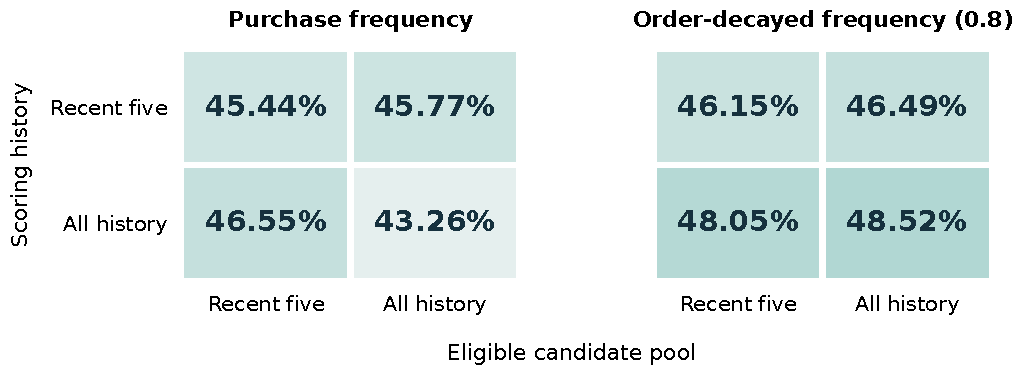
\includegraphics[width=\linewidth]{factorial_memory.pdf}
  \caption{Factorial comparison on the same 2,526 users with at least 16 historical orders and nonempty repeat targets. Rows change scoring history and columns change candidate eligibility. All cells use the complete historical catalog and fixed repeat-target denominator. Values are macro Recall@10.}
  \label{fig:factorial}
\end{figure}

\begin{table}[tbp]
  \centering
  \caption{All nine prespecified main-study contrasts. Differences and intervals are in percentage points of Recall@10. Intervals are simultaneous 95\% over the nine contrasts. The noninferiority claim concerns the selected-minus-full row and the predeclared $-0.5\pp$ margin.}
  \label{tab:primary}
  \small
  \begin{tabular}{@{}lrrr@{}}
    \toprule
    Contrast & Users & Difference & Simultaneous 95\% interval \\
    \midrule
    Frequency scoring information & 2,526 & $-2.513$ & $[-3.846,-1.163]$ \\
    Decay scoring information & 2,526 & $+2.030$ & $[+1.291,+2.734]$ \\
    Frequency candidate expansion & 2,526 & $-3.287$ & $[-4.356,-2.265]$ \\
    Decay candidate expansion & 2,526 & $+0.466$ & $[+0.139,+0.826]$ \\
    Frequency interaction & 2,526 & $-3.624$ & $[-4.639,-2.630]$ \\
    Decay interaction & 2,526 & $+0.130$ & $[-0.172,+0.435]$ \\
    \midrule
    Selected minus full & 7,472 & $+0.007$ & $[-0.066,+0.071]$ \\
    Selected minus frequency budget & 7,472 & $+0.192$ & $[+0.044,+0.342]$ \\
    Selected minus recency budget & 7,472 & $+0.061$ & $[-0.039,+0.165]$ \\
    \bottomrule
  \end{tabular}
\end{table}

The exact ledger in Table~\ref{tab:ledger} explains the net change. Frequency retrieves some old true targets, but loses more recall through displaced correct recommendations. Decay introduces fewer old products into the leading positions and achieves a positive balance. These observations reject a blanket recommendation to discard all older products. The frequency interaction is negative, while the decay interaction interval includes zero. Because recent scoring assigns zero to old products, part of the interaction is structural. We therefore emphasize fixed-score candidate expansion. The learned-model ledger is descriptive rather than an additional prespecified test.

\begin{table}[tbp]
  \centering
  \caption{Exact hit accounting for expansion from recent candidates to all historical candidates under fixed full-history scores. Each contribution is divided by the same user's full repeat-target count before averaging across the 2,526 long-history users. Learned-model contributions average three seeds. Displayed rounding can affect sums; stored per-user identities balance exactly.}
  \label{tab:ledger}
  \small
  \begin{tabularx}{\linewidth}{@{}Xrrr@{}}
    \toprule
    Scoring method & Recovered true hits & Displaced true hits & Net recall \\
    \midrule
    Frequency & $+3.66\pp$ & $-6.94\pp$ & $-3.29\pp$ \\
    Decay & $+0.61\pp$ & $-0.14\pp$ & $+0.47\pp$ \\
    Learned model & $+1.45\pp$ & $-0.58\pp$ & $+0.87\pp$ \\
    \bottomrule
  \end{tabularx}
\end{table}

\subsection{Selective retention preserves short-list performance}
Validation selects $M=5$: recent-only candidates fail the selection criterion, and adding up to five older frequent products gives the smallest tested qualifying pool. Selection, model scores, and evaluation code are frozen before confirmation. Table~\ref{tab:policies} reports the independent confirmation outcomes for this fixed policy and its controls.

\begin{table}[tbp]
  \centering
  \caption{Candidate policies on the memory-study confirmation cohort. Candidate means use all 8,000 users; Recall@10 and target coverage use the 7,472 nonempty-target users. Same-budget controls match the selected pool size separately for every user.}
  \label{tab:policies}
  \small
  \begin{tabularx}{\linewidth}{@{}Xrrr@{}}
    \toprule
    Candidate policy & Mean candidates & Recall@10 & Target coverage \\
    \midrule
    Full historical pool & 64.92 & 58.164\% & 100.00\% \\
    Recent five orders only & 32.49 & 57.674\% & 87.06\% \\
    Recent plus five old frequent & 35.85 & 58.171\% & 90.87\% \\
    Same-budget frequency & 35.85 & 57.980\% & 89.91\% \\
    Same-budget recency & 35.85 & 58.110\% & 90.48\% \\
    \bottomrule
  \end{tabularx}
\end{table}

Total eligible candidate volume decreases by 44.79\%, equivalently the reduction in the ratio of mean candidate counts for the same 8,000 users. The mean of users' individual retention ratios is 73.01\%, a different aggregation. Selected-minus-full recall is $+0.0072\pp$, with simultaneous interval $[-0.0657,+0.0713]\pp$. Its lower bound exceeds the prespecified $-0.5\pp$ margin, supporting noninferiority. The interval crosses zero, so the evidence does not establish superiority or exact equality.

\begin{figure}[tbp]
  \centering
  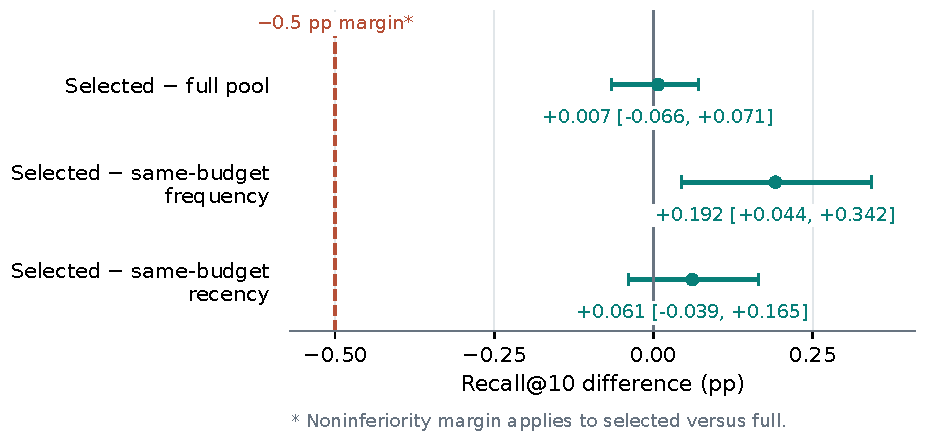
\includegraphics[width=0.95\linewidth]{policy_contrasts.pdf}
  \caption{Main-study policy contrasts on 7,472 nonempty-target users. Bars show simultaneous 95\% intervals across the nine prespecified contrasts. The $-0.5\pp$ reference applies to selected versus full noninferiority; it is not a superiority threshold for all contrasts.}
  \label{fig:policies}
\end{figure}

The selected policy exceeds same-budget frequency by $0.192\pp$, but the $0.061\pp$ difference from same-budget recency is uncertain. The result therefore supports selective retention under the tested conditions, without showing that the old-frequency rule is uniquely optimal.

\paragraph{Recall retention does not preserve all target coverage.}
Macro candidate coverage falls to 90.87\%, and the candidate-constrained oracle Recall@10 decreases from 93.34\% to 86.09\%. Excluded true targets remain in evaluation, but the current full ranker rarely retrieves them in its Top~10. Coverage loss and nearly unchanged achieved recall can consequently coexist. This does not mean the excluded products lack value.

The full model's whole-basket Recall@10 is 35.82\%, compared with 58.16\% for repeat targets. First-time product recommendation is outside this study's modeled candidate scope. In addition, full scores are computed before candidate masking, so candidate reduction does not demonstrate faster scoring, lower memory use, or end-to-end deployment savings.

\subsection{Posthoc interpretation and recommendation-depth limits}
\label{sec:posthoc}
After confirmation, we inspect the frozen predictions without fitting models or choosing new parameters. All findings in this subsection are posthoc. Among 7,472 users with nonempty repeat targets, 7,431 (99.45\%) have unchanged seed-averaged recall, 23 improve, and 18 decline. Across all 8,000 users, 96.225\% retain exactly the same ordered Top~10 under all three models. Average preservation therefore arises mainly from unchanged recommendations, rather than broad gains offsetting broad losses.

Some individuals still lose: the 18 harmed users have a conditional mean recall decline of $21.03\pp$. This outcome-selected group is not a validated prediction-time subgroup. Historical subgroup intervals do not supply stable evidence for a deployment subgroup that reliably benefits.

Of 5,274 excluded true repeat targets, only 0.26\% originally rank in the full model's Top~10, while 95.54\% rank after position 20, averaging rank-bin counts across seeds. Longer full-pool lists begin to reach these targets, making deletion losses exceed gains from promoted retained products. Figure~\ref{fig:depth} and Table~\ref{tab:depth} show all six inspected list lengths. The twelve posthoc contrasts use a separate family of simultaneous intervals; the repeated $K=10$ point is not another independent confirmation.

\begin{figure}[tbp]
  \centering
  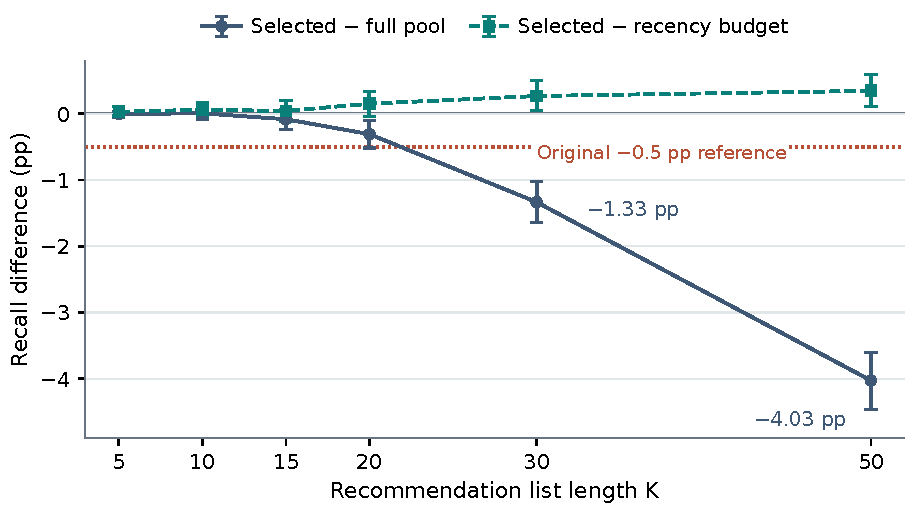
\includegraphics[width=0.95\linewidth]{list_depth.pdf}
  \caption{Posthoc recommendation-depth analysis. Policies and scores are fixed. Intervals use 6,000 paired-user bootstrap samples and simultaneous adjustment over twelve comparisons. Lines connect tested values only. The original $-0.5\pp$ margin is a reference, not a newly confirmed safe-$K$ boundary.}
  \label{fig:depth}
\end{figure}

\begin{table}[tbp]
  \centering
  \caption{All twelve posthoc depth contrasts on 7,472 nonempty-target users. Each entry reports selected-minus-comparator Recall@K in percentage points, followed by its simultaneous 95\% interval. These intervals belong to the posthoc family and differ from the original nine-contrast confirmation intervals.}
  \label{tab:depth}
  \small
  \begin{tabular}{@{}rcc@{}}
    \toprule
    $K$ & Compared with full pool & Compared with recency budget \\
    \midrule
    5  & $-0.001\;[-0.057,+0.042]$ & $+0.032\;[-0.028,+0.115]$ \\
    10 & $+0.007\;[-0.078,+0.070]$ & $+0.061\;[-0.047,+0.172]$ \\
    15 & $-0.082\;[-0.241,+0.070]$ & $+0.043\;[-0.114,+0.201]$ \\
    20 & $-0.308\;[-0.517,-0.103]$ & $+0.152\;[-0.036,+0.336]$ \\
    30 & $-1.334\;[-1.645,-1.023]$ & $+0.269\;[+0.045,+0.497]$ \\
    50 & $-4.028\;[-4.471,-3.606]$ & $+0.349\;[+0.106,+0.592]$ \\
    \bottomrule
  \end{tabular}
\end{table}

At $K=20$, the selected-minus-full interval $[-0.517,-0.103]\pp$ slightly crosses the original margin. This does not overturn the original Top~10 confirmation, and these posthoc observations do not establish a newly chosen safe cutoff. At $K=30$ and 50, losses increase to $1.334$ and $4.028\pp$.

The recency-budget control remains close partly because both policies retain all recent products. Their overall candidate Jaccard averages 92.92\%, versus 53.35\% for old-only candidates among users with a nonempty old union. For 94.61\% of all users, all three models produce identical Top~10 lists. At $K=30$ and 50, selected retention modestly exceeds recency-budget recall but still falls behind the full pool. These local advantages do not establish overall superiority, and low original ranks do not imply that a stronger model could never recover the excluded targets.
